% `template.tex', a bare-bones example employing the AIAA class.
%
% For a more advanced example that makes use of several third-party
% LaTeX packages, see `advanced_example.tex', but please read the
% Known Problems section of the users manual first.
%
% Typical processing for PostScript (PS) output:
%
%  latex template
%  latex template   (repeat as needed to resolve references)
%
%  xdvi template    (onscreen draft display)
%  dvips template   (postscript)
%  gv template.ps   (onscreen display)
%  lpr template.ps  (hardcopy)
%
% With the above, only Encapsulated PostScript (EPS) images can be used.
%
% Typical processing for Portable Document Format (PDF) output:
%
%  pdflatex template
%  pdflatex template      (repeat as needed to resolve references)
%
%  acroread template.pdf  (onscreen display)
%
% If you have EPS figures, you will need to use the epstopdf script
% to convert them to PDF because PDF is a limmited subset of EPS.
% pdflatex accepts a variety of other image formats such as JPG, TIF,
% PNG, and so forth -- check the documentation for your version.
%
% If you do *not* specify suffixes when using the graphicx package's
% \includegraphics command, latex and pdflatex will automatically select
% the appropriate figure format from those available.  This allows you
% to produce PS and PDF output from the same LaTeX source file.
%
% To generate a large format (e.g., 11"x17") PostScript copy for editing
% purposes, use
%
%  dvips -x 1467 -O -0.65in,0.85in -t tabloid template
%
% For further details and support, read the Users Manual, aiaa.pdf.


% Try to reduce the number of latex support calls from people who
% don't read the included documentation.
%


\typeout{}\typeout{If latex fails to find aiaa-tc, read the README file!}
%


\documentclass[]{aiaa-tc}% insert '[draft]' option to show overfull boxes
\usepackage{float}
\usepackage{epstopdf}
\usepackage{amsmath}
\usepackage[table,xcdraw]{xcolor}

\title{Advanced Astrodynamics HW3}

\author{
	Johnathan Clouse%
	\thanks{Graduate Student, Aerospace Engineering Sciences, 1111 Engineering Drive, Boulder, CO, 80309-0429}\\
	{\normalsize\itshape
		University of Colorado, Boulder, CO, 80309-0429, USA}
}

% Define commands to assure consistent treatment throughout document
\newcommand{\eqnref}[1]{(\ref{#1})}
\newcommand{\class}[1]{\texttt{#1}}
\newcommand{\package}[1]{\texttt{#1}}
\newcommand{\file}[1]{\texttt{#1}}
\newcommand{\BibTeX}{\textsc{Bib}\TeX}

\usepackage[euler]{textgreek}
\usepackage[colorlinks=true]{hyperref}
\hypersetup{urlcolor=cyan}

\usepackage{listings}
\usepackage{color} %red, green, blue, yellow, cyan, magenta, black, white
\definecolor{mygreen}{RGB}{28,172,0} % color values Red, Green, Blue
\definecolor{mylilas}{RGB}{170,55,241}

\usepackage{tablefootnote}
\usepackage{graphicx}
\usepackage{amsmath}
\usepackage{bm}
\usepackage{subfigure}
%\usepackage{subcaption}

\definecolor{mylilas}{RGB}{170,55,241}

% See p.105 of "TeX Unbound" for suggested values.
% See pp. 199-200 of Lamport's "LaTeX" book for details.
%   General parameters, for ALL pages:
\renewcommand{\topfraction}{0.9}	% max fraction of floats at top
\renewcommand{\bottomfraction}{0.8}	% max fraction of floats at bottom
%   Parameters for TEXT pages (not float pages):
\setcounter{topnumber}{2}
\setcounter{bottomnumber}{2}
\setcounter{totalnumber}{4}     % 2 may work better
\setcounter{dbltopnumber}{2}    % for 2-column pages
\renewcommand{\dbltopfraction}{0.9}	% fit big float above 2-col. text
\renewcommand{\textfraction}{0.07}	% allow minimal text w. figs
%   Parameters for FLOAT pages (not text pages):
\renewcommand{\floatpagefraction}{0.7}	% require fuller float pages
% N.B.: floatpagefraction MUST be less than topfraction !!
\renewcommand{\dblfloatpagefraction}{0.7}	% require
    \makeatletter
    \renewcommand\l@section{\@dottedtocline{2}{1.5em}{3em}}
    \makeatother
    
\begin{document}
	

	
	\maketitle
	
	\begin{abstract}
		\noindent 
		
	\end{abstract}
	
	\newpage
	
	\tableofcontents
	
	\newpage
	\section{Problem 14}
Due to the given initial conditions, there will be no z-component to the motion. This means that the right-ascention, the argument of periapsis, and true anomaly are not well-defined; they are combined into the longitude of periapsis. 


	\begin{figure}[H]
		\centering
		\subfigure[Position]{
			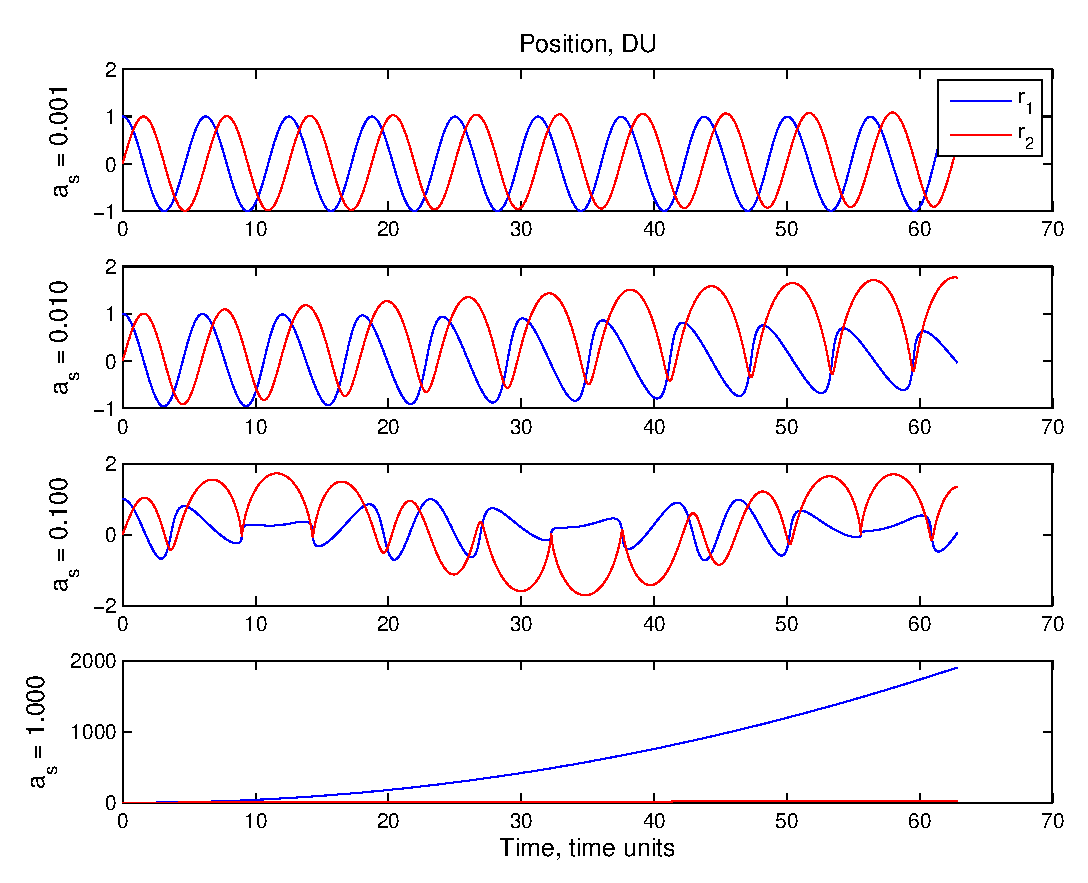
\includegraphics[width = 10cm]{Figures/P14_R.eps}
		}
		\subfigure[Velocity]{
			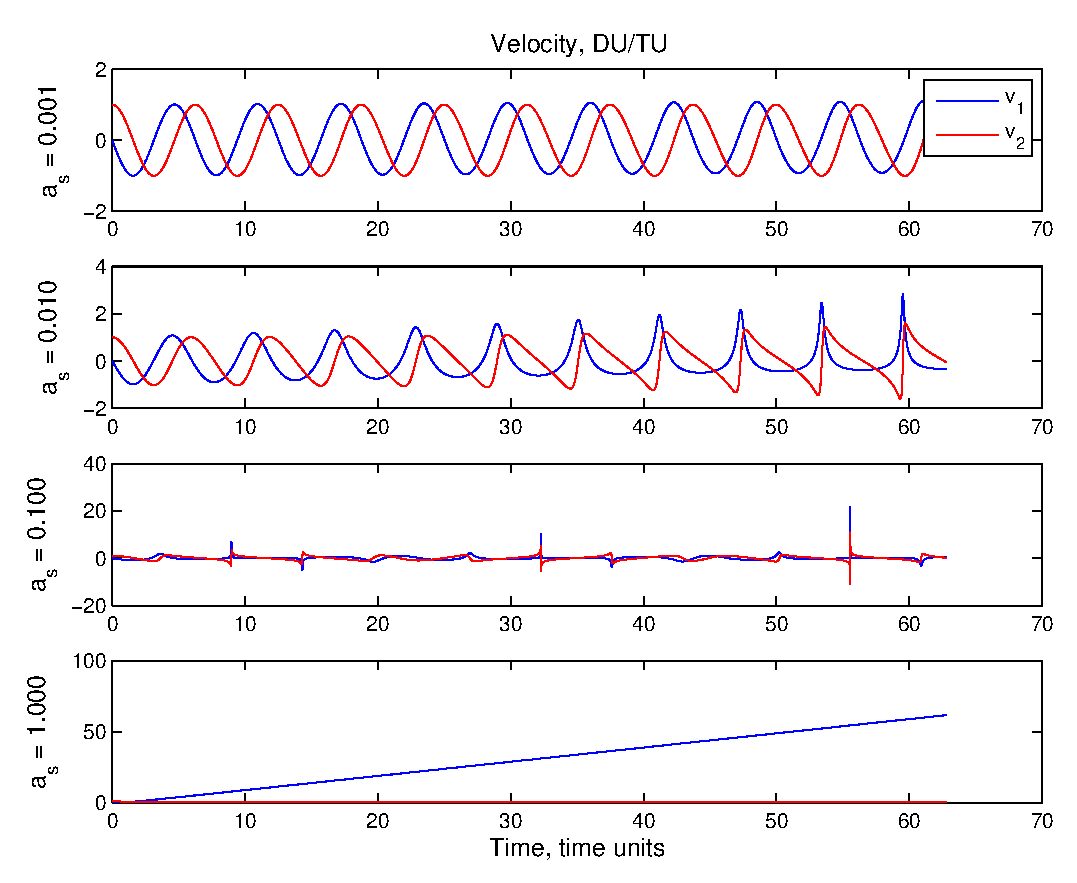
\includegraphics[width = 10cm]{Figures/P14_V.eps}
		}
	\caption{Simulation results, cartesian elements }
		\label{fig:P14_cart}
	\end{figure}	

	\begin{figure}[H]
		\centering
		\subfigure[Semimajor axis]{
			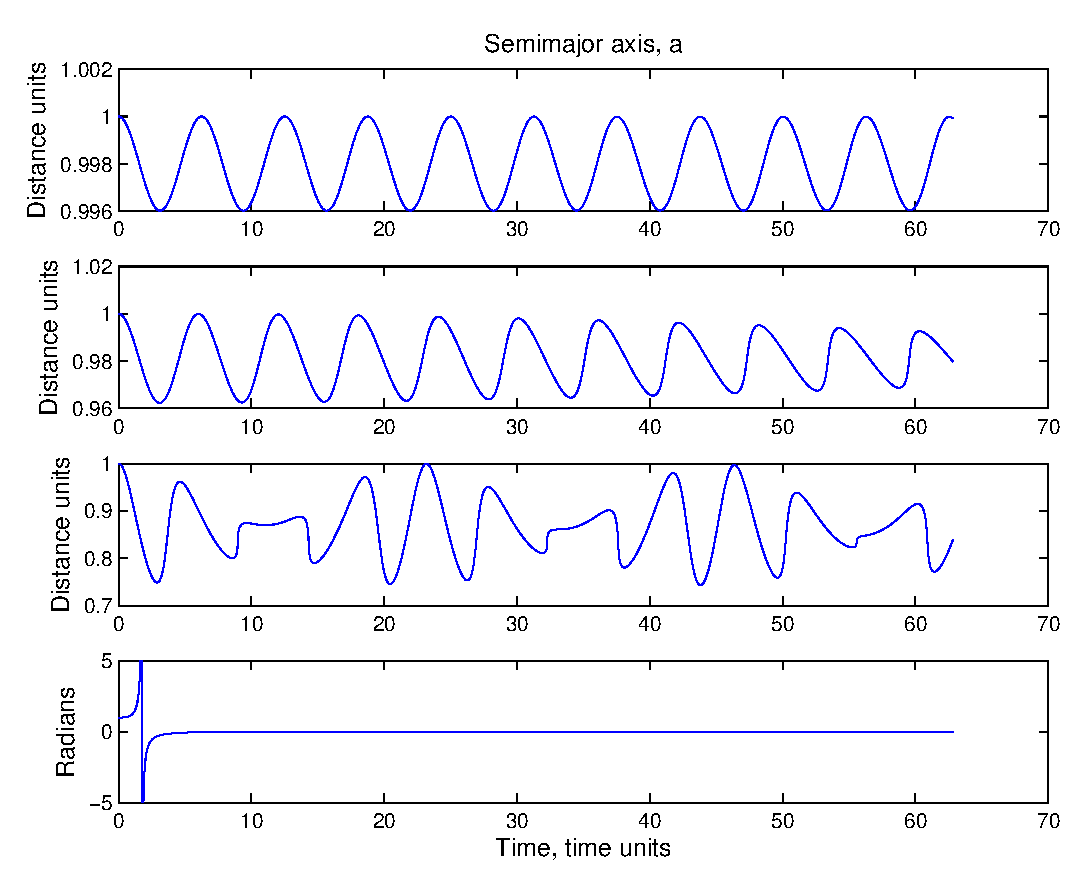
\includegraphics[width = 7.5cm]{Figures/P14_SMA.eps}
		}
		\subfigure[Eccentricity]{
			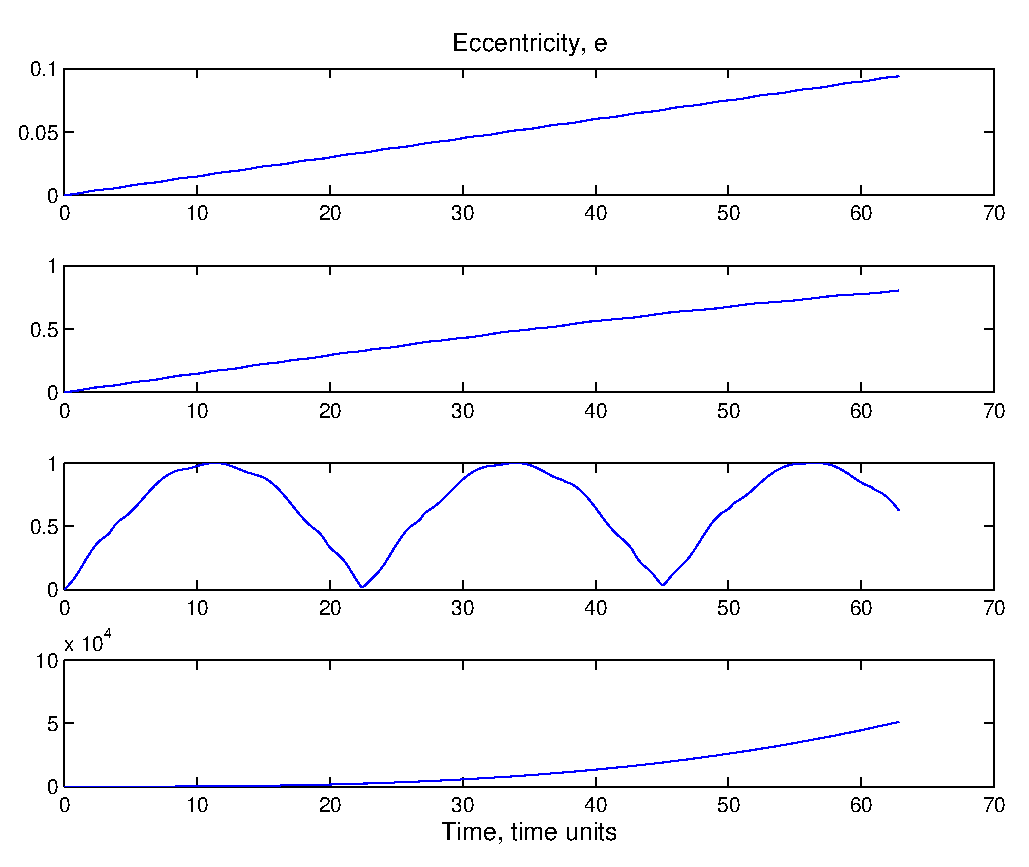
\includegraphics[width = 7.5cm]{Figures/P14_Ecc.eps}
		}
		\subfigure[Inclination]{
			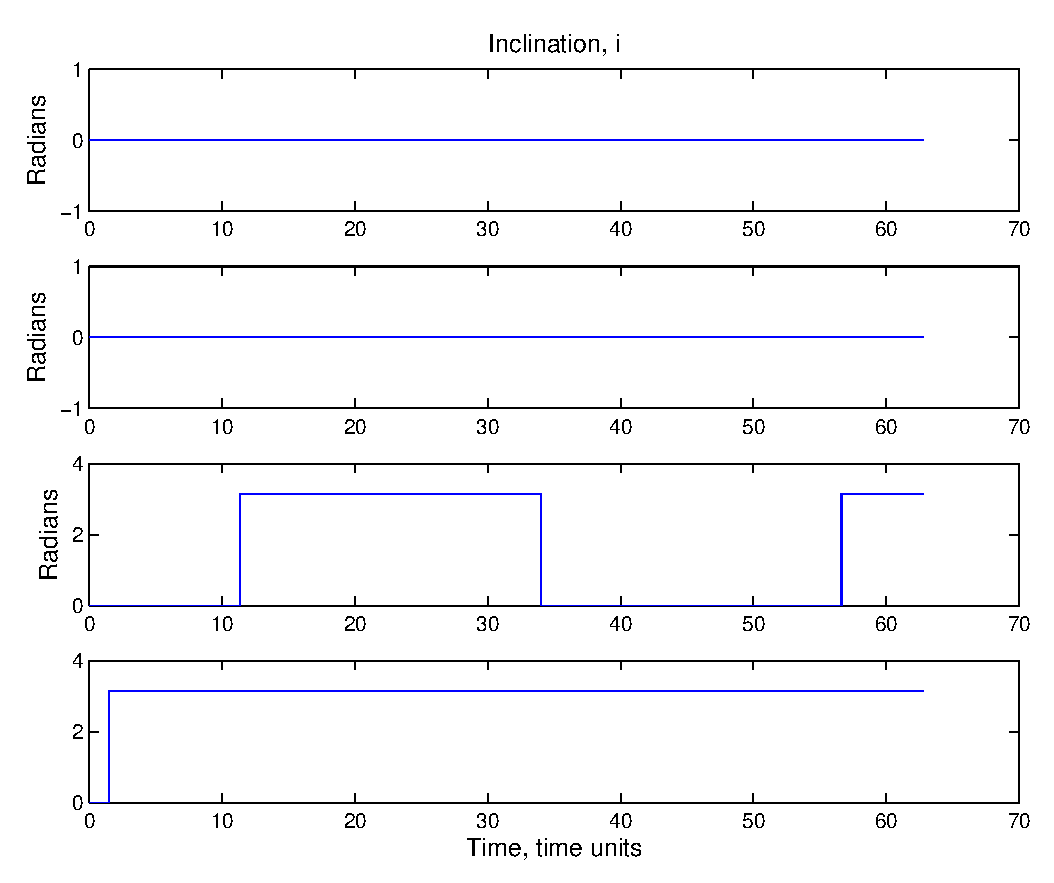
\includegraphics[width = 7.5cm]{Figures/P14_i.eps}
		}
		\subfigure[Argument of periapsis]{
			\includegraphics[width = 7.5cm]{Figures/P14_w.eps}
		}
		\subfigure[RAAN]{
			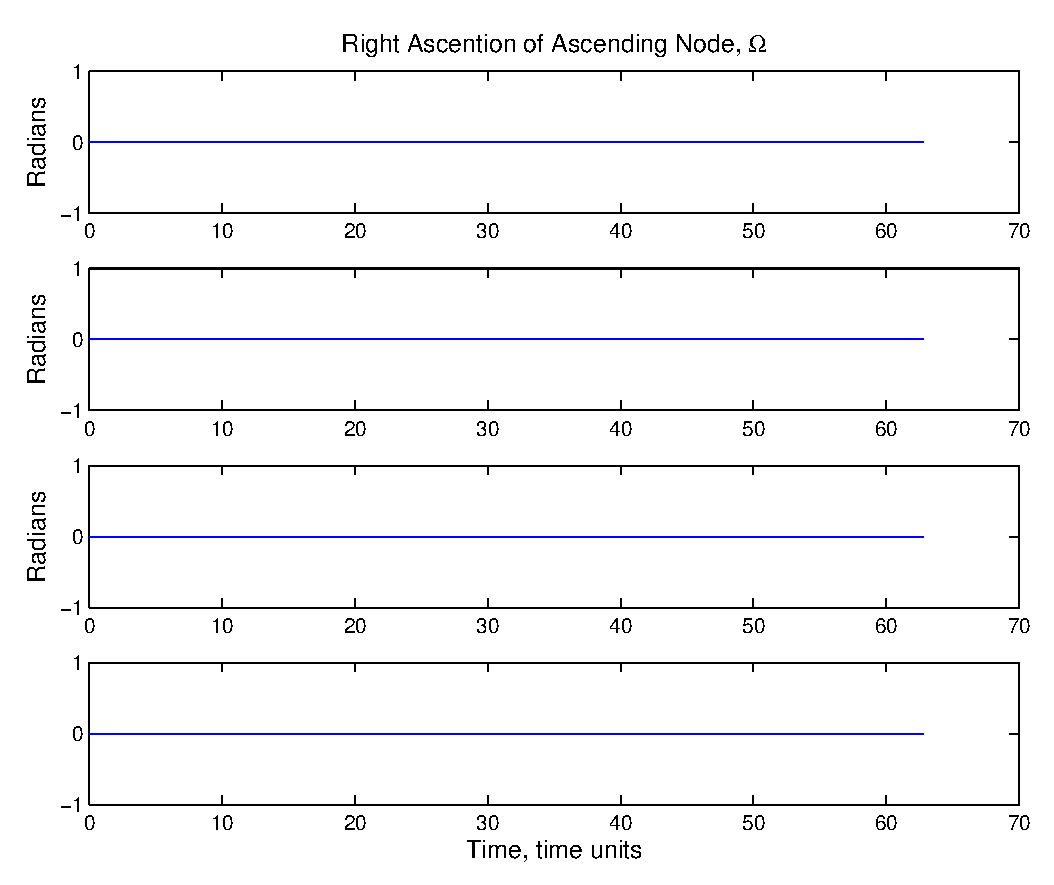
\includegraphics[width = 7.5cm]{Figures/P14_RAAN.eps}
		}
		\subfigure[Longitude of periapsis]{
			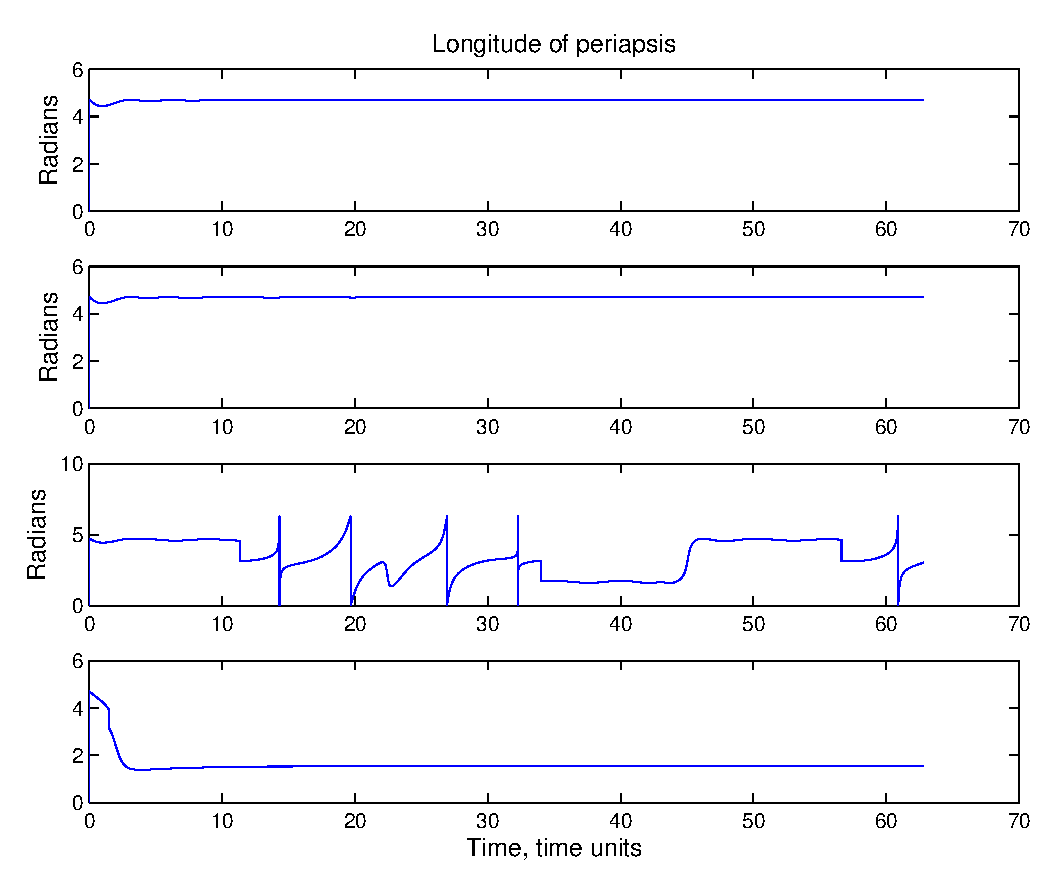
\includegraphics[width = 7.5cm]{Figures/P14_f.eps}
		}
	\caption{Simulation results, orbital elements }
		\label{fig:P14_OE}
	\end{figure}	

For the cartesian elements, the third components were zero due to the initial conditions and the perturbation acceleration. In the lowest acceleration case, the case stays close to circular and is evident to the components being about 90$^\circ$ out of phase. The second case has even more pronounced effects that take the motion from sinusoidal to almost a sine wave. The third case has an acceleration large enough to take the orbiter close to the origin; the inclination plot shows in this case that the orbit flips between retrograde and prograde.  In the final case, the orbiter escapes and the x component grows significantly due to the perturbation acceleration in that direction.

For the orbital elements, one can see the first two cases are prograde with increasing eccentricity. Interestingly, the osculating longitude of periapsis for both cases converges to some value, instead of varying sinusoidally between 0 and 2$\pi$. This means the osculating orbit is rotating with the orbiter. For the third case, the orbit switches between prograde and retrograde when the eccentricy hits 1. The perturbation acceleration is just enough to reverse to orbit direction, but not enough to cancel out the acceleration due to the primary body. Finally, the last case shows a transition to a hyperbolic orbit. There is a discontinuity in $a$ when the transition happens, going to infinity (parabolic trajectory) and then negative (hyperbolic). The $e<1$ confirms this result. 

	\section{Problem 15}
Many of the derivations in this problem include integrals of trigonomic functions of the eccentric anomaly $E$. They are derived here to make subsequent derivations cleaner.
	\begin{equation}
		\int_{0}^{2\pi}\textup{cos}EdE=\textup{sin}E\rvert_{0}^{2\pi}=\textup{sin}2\pi-\textup{sin}0=0-0=0
		\label{eqn:cosInt}
	\end{equation}
	\begin{equation}
		\int_{0}^{2\pi}\textup{sin}EdE=-\textup{cos}E\rvert_{0}^{2\pi}=-(\textup{cos}2\pi-\textup{cos}0)=-1+1=0
		\label{eqn:sinInt}
	\end{equation}
For the integral of $\textup{cos}^2E$, the substitution $u=2E$ is used:
	\begin{equation}
		\int_{0}^{2\pi}\textup{cos}^2EdE=\int_{0}^{2\pi}\frac{1+ \textup{cos} 2E }{2}dE=\int_{0}^{2\pi}\frac{1}{2}dE+\int_{0}^{\pi}\frac{1}{4}\textup{cos}udu=\left [\frac{E}{2}+\frac{\textup{sin} 2E}{4}  \right ]_0^{2\pi}=\pi
		\label{eqn:cos2Int}
	\end{equation}
For the integral of $\textup{cos}E\textup{sin}E$, the substitution $u=\textup{cos}E$ is used:
	\begin{equation}
		\int_{0}^{2\pi}\textup{cos}E\textup{sin}EdE=-\int_{E=0}^{E=2\pi}udu=-\frac{u^2}{2}\bigg|_{E=0}^{E=2\pi}=-\frac{\textup{cos}^2E}{2}\bigg|_{E=0}^{E=2\pi}=-\frac{(1-1)}{2}=0
		\label{eqn:cosSinInt}
	\end{equation}
And finally, the simplest integral of them all:
	\begin{equation}
\int_{0}^{2\pi}dE=E\bigg|_0^{2\pi}=2\pi
		\label{eqn:EInt}
	\end{equation}
\subsection {}
For 
$R$ in terms of $E$, separate $\omega$ and $f$ and convert to the eccentric anomaly:
	\begin{equation}
		R = \frac{a(1-e^2)}{1+e\textup{cos}f}\textup{sin}i(\textup{sin}\omega \textup{cos}f+\textup{cos}\omega \textup{sin}f)a_s
	\end{equation}
	\begin{equation}
		R =a(1-e\textup{cos}E)\textup{sin}i(\textup{sin}\omega \frac{\textup{cos}E-e}{(1-e\textup{cos}E)}+\textup{cos}\omega \frac{\sqrt{1-e^2}\textup{sin}E}{(1-e\textup{cos}E)})a_s
	\end{equation}
	\begin{equation}
		R = a\textup{sin}i(-e\textup{sin}\omega+\textup{sin}\omega \textup{cos}E +\sqrt{1-e^2}\textup{cos}\omega\textup{sin}E )a_s
	\end{equation}

The averaging operator is defined as:
	\begin{equation}
		\bar{g} = \frac{1}{2\pi}\ \int_{0}^{2\pi}g(M)dM= \frac{1}{2\pi}\ \int_{0}^{2\pi}g(E)(1-e\textup{cos}E)dE
		\label{eqn:avg_operator}
	\end{equation}
Applying the operator to the potential function for the mean potential over one orbit:
	\begin{equation}
		\bar{R} = \frac{1}{2\pi}\ \int_{0}^{2\pi} a\textup{sin}i(-e\textup{sin}\omega+\textup{sin}\omega \textup{cos}E +\sqrt{1-e^2}\textup{cos}\omega\textup{sin}E )a_s(1-e\textup{cos}E)dE
	\end{equation}
	\begin{equation}
		\bar{R} = \frac{aa_s\textup{sin}i}{2\pi}\ \int_{0}^{2\pi} (-e\textup{sin}\omega+\textup{sin}\omega \textup{cos}E +\sqrt{1-e^2}\textup{cos}\omega\textup{sin}E +e^2\textup{sin}\omega\textup{cos}E-e\textup{sin}\omega \textup{cos}^2E-e\sqrt{1-e^2}\textup{cos}\omega\textup{sin}E\textup{cos}E)dE
	\end{equation}

Substituting the integrals from Eqns \ref{eqn:cosInt}, \ref{eqn:sinInt}, \ref{eqn:cos2Int}, \ref{eqn:cosSinInt}, and \ref{eqn:EInt}:
	\begin{equation}
		\bar{R} = \frac{aa_s\textup{sin}i}{2\pi}\  (-e\textup{sin}\omega[2\pi+\pi])=-\frac{3}{2}ae\textup{sin} \omega \textup{sin}i\,   a_s 
	\end{equation}


\subsection {}

The Lagrange equations for $a$ and $e$ are generally:
	\begin{equation}
		\dot{a}=\frac{2}{na}\frac{\partial R}{\partial \sigma} 
		\label{eqn:a_dot_gen}
	\end{equation}
	\begin{equation}
		\dot{e}=\frac{1}{na^2e}\left [ (1-e^2)\frac{\partial R}{\partial \sigma}  - \sqrt{1-e^2}\frac{\partial R}{\partial \omega} \right]
		\label{eqn:e_dot_gen}
	\end{equation}

The quantity $\frac{\partial R}{\partial \sigma}$ needs to be found by use of the chain rule, so that $\frac{\partial R}{\partial \sigma} = \frac{\partial R}{\partial f}\frac{\partial f}{\partial E}\frac{\partial E}{\partial \sigma}$. Start with $\frac{\partial E}{\partial \sigma}$ by taking the relation between $M$ and $E$ 

	\begin{equation}
		M=nt+\sigma=E-e\textup{sin}E 
	\end{equation}
and taking the partial derivative with respect to $\sigma$:
	\begin{equation}
		1=\frac{\partial E}{\partial \sigma}-e\frac{\partial E}{\partial \sigma}\textup{cos}E 
	\end{equation}
	\begin{equation}
		\frac{\partial E}{\partial \sigma}=\frac{1}{1-e\textup{cos}E}=\frac{a}{r}=\frac{1+e\textup{cos}f}{1-e^2}
		\label{eqn:partialESig}
	\end{equation}

For $\frac{\partial f}{\partial E}$ take the relation between $E$ and $f$ 
	\begin{equation}
		\textup{tan}\frac{1}{2}E=\sqrt{\frac{1-e}{1+e}}\textup{tan}\frac{1}{2}f
	\end{equation}
and take the partial derivative with respect to $E$:
	\begin{equation}
		\frac{1}{2}\textup{sec}^2\frac{1}{2}E=\frac{\partial f}{\partial E}\sqrt{\frac{1-e}{1+e}}\frac{1}{2}\textup{sec}^2\frac{1}{2}f
	\end{equation}
Solve for $\frac{\partial f}{\partial E}$:
	\begin{equation}
		\frac{\partial f}{\partial E} = \sqrt{\frac{1+e}{1-e}}\frac{\textup{sec}^2\frac{1}{2}E}{\textup{sec}^2\frac{1}{2}f}= \sqrt{\frac{1+e}{1-e}}\frac{\textup{cos}^2\frac{1}{2}f}{\textup{cos}^2\frac{1}{2}E}
	\end{equation}

Using the identity $\textup{cos}^2\frac{1}{2}x=\frac{1+{cos}x}{2}$:
	\begin{equation}
		\frac{\partial f}{\partial E} = \sqrt{\frac{1+e}{1-e}}\frac{1+\textup{cos}f}{1+\textup{cos}E}\sqrt{\frac{1+e}{1+e}}=\frac{\left ( 1+e \right )\left (1+\textup{cos}f  \right )}{\sqrt{1-e^2}\left (1+\textup{cos}E  \right )}=\frac{1+e\textup{cos}f+e+\textup{cos}f}{\sqrt{1-e^2}\left (1+\textup{cos}E  \right )}
	\end{equation}
	\begin{equation}
		\frac{\partial f}{\partial E} =\frac{ \left [\frac{1+e\textup{cos}f}{1+e\textup{cos}f}+\frac{e+\textup{cos}f }{1+e\textup{cos}f}  \right ]\left (1+e\textup{cos}f  \right )}{\sqrt{1-e^2}\left (1+\textup{cos}E  \right )}
	\end{equation}
	\begin{equation}
		\frac{\partial f}{\partial E} =\frac{ \left (1+\textup{cos}E  \right )\left (1+e\textup{cos}f  \right )}{\sqrt{1-e^2}\left (1+\textup{cos}E  \right )}=\frac{ 1+e\textup{cos}f }{\sqrt{1-e^2}}
		\label{eqn:partialfE}
	\end{equation}

 $\frac{\partial R}{\partial f}$ is found through the derivative quotient rule and simplifying:
	\begin{equation}
		\frac{\partial R}{\partial f}=\frac{\partial }{\partial f}\left ( \frac{a(1-e^2)}{1+e\textup{cos}f}\textup{sin}i \textup{sin}(\omega +f ) \, a_s\right )= a(1-e^2)\textup{sin}i\, a_s\left [ \frac{\textup{cos}(\omega +f )\left (1+e\textup{cos}f  \right )-(-e\textup{sin}f)\textup{sin}(\omega +f )}{\left (1+e\textup{cos}f  \right )^2} \right ]
	\end{equation}
Simplifying the bracketed quantity, assigned to $A$:
	\begin{equation}
		\begin{aligned}
 A &= \frac{\textup{cos}(\omega +f )\left (1+e\textup{cos}f  \right )-(-e\textup{sin}f)\textup{sin}(\omega +f )}{\left (1+e\textup{cos}f  \right )^2} \\
&= \frac{\textup{cos}(\omega +f )+e\textup{cos}f\textup{cos}(\omega +f ) +e\textup{sin}f\textup{sin}(\omega +f )}{\left (1+e\textup{cos}f  \right )^2}\\ 
 &= \frac{\textup{cos}(\omega +f )+e\textup{cos}f(\textup{cos}\omega\textup{cos}f - \textup{sin}\omega\textup{sin}f) +e\textup{sin}f(\textup{sin}\omega\textup{cos}f+\textup{cos}\omega\textup{sin}f)}{\left (1+e\textup{cos}f  \right )^2}\\ 
 &= \frac{\textup{cos}(\omega +f )+e\textup{cos}^2f\textup{cos}\omega - e\textup{sin}\omega\textup{sin}f\textup{cos}f +e\textup{sin}\omega\textup{sin}f\textup{cos}f+e\textup{cos}\omega\textup{sin}^2f)}{\left (1+e\textup{cos}f  \right )^2} \\
 &= \frac{\textup{cos}(\omega +f )+e\textup{cos}\omega}{\left (1+e\textup{cos}f  \right )^2} \\
\end{aligned}
	\end{equation}
Which makes the desired partial
	\begin{equation}
\frac{\partial R}{\partial f}= a(1-e^2)\textup{sin}i\, a_s\left [\frac{\textup{cos}(\omega +f )+e\textup{cos}\omega}{\left (1+e\textup{cos}f  \right )^2}  \right ] 
	\label{eqn:partialRf}
	\end{equation}

Now we have $\frac{\partial R}{\partial \sigma}$ through Equations \ref{eqn:partialESig}, \ref{eqn:partialfE}, and \ref{eqn:partialRf}:
	\begin{equation}
\begin{aligned}
\frac{\partial R}{\partial \sigma}= \frac{\partial R}{\partial f}\frac{\partial f}{\partial E}\frac{\partial E}{\partial \sigma}&=a(1-e^2)\textup{sin}i\, a_s\left [\frac{\textup{cos}(\omega +f )+e\textup{cos}\omega}{\left (1+e\textup{cos}f  \right )^2}  \right ] \frac{ 1+e\textup{cos}f }{\sqrt{1-e^2}}\frac{1+e\textup{cos}f}{1-e^2} \\
&=\frac{a}{\sqrt{1-e^2}}\textup{sin}i \left [ \textup{cos}(\omega +f )+e\textup{cos}\omega \right ]a_s
 \end{aligned}
	\label{eqn:partialRSig}
	\end{equation}

Equation \ref{eqn:a_dot_gen} becomes
\begin{equation}
\begin{aligned} 
\dot{a} &= \frac{2}{na}\frac{a}{\sqrt{1-e^2}}\textup{sin}i \left [ \textup{cos}(\omega +f )+e\textup{cos}\omega \right ]a_s \\
 &=\frac{2}{n\sqrt{1-e^2}}\textup{sin}i \left [ \textup{cos}(\omega +f )+e\textup{cos}\omega \right ]a_s
\end{aligned}
	\end{equation}

Finding $\frac{\partial R}{\partial \omega}$ to be
	\begin{equation}
\frac{\partial R}{\partial \omega}=\frac{\partial }{\partial \omega}\left ( ra_s\textup{sin}i\textup{sin}(\omega+f)) \right )=ra_s\textup{sin}i\textup{cos}(\omega+f))
	\label{eqn:a_dot} 
	\end{equation}

equation \ref{eqn:e_dot_gen} becomes
	\begin{equation}
\begin{aligned} 
\dot{e} &= \frac{1}{na^2e}\left [ (1-e^2) \left [\frac{a}{\sqrt{1-e^2}}\textup{sin}i \left [ \textup{cos}(\omega +f )+e\textup{cos}\omega \right ]a_s\right ]  - \sqrt{1-e^2}\left [ra_s\textup{sin}i\textup{cos}(\omega+f))  \right ] \right] \\
 &= \frac{\sqrt{1-e^2}\textup{sin}i}{na}\, a_s\left [ \frac{\textup{cos}(\omega +f )}{e} +\textup{cos}\omega -\frac{\textup{cos}(\omega +f )}{e}\frac{1-e^2}{1+e\textup{cos}f}\right ] \\
 &= \frac{\sqrt{1-e^2}\textup{sin}i}{na}\, a_s\left [ \textup{cos}\omega +\frac{\textup{cos}(\omega +f )}{e}\left [1-\frac{1-e^2}{1+e\textup{cos}f}  \right ]\right ] \\
 &= \frac{\sqrt{1-e^2}\textup{sin}i}{na}\, a_s\left [ \textup{cos}\omega +\frac{\textup{cos}(\omega +f )}{e}\left [\frac{1+e\textup{cos}f}{1+e\textup{cos}f}-\frac{1-e^2}{1+e\textup{cos}f}  \right ]\right ] \\
 &= \frac{\sqrt{1-e^2}\textup{sin}i}{na}\, a_s\left [ \textup{cos}\omega +\frac{\textup{cos}(\omega +f )}{e}\frac{e(e+\textup{cos}f)}{1+e\textup{cos}f}\right ] \\
\end{aligned}
	\end{equation}
	\begin{equation}
\dot{e}= \frac{\sqrt{1-e^2}\textup{sin}i}{na}\, a_s\left [ \textup{cos}\omega +\textup{cos}(\omega +f )\frac{(e+\textup{cos}f)}{1+e\textup{cos}f}\right ]  
	\label{eqn:e_dot} 
	\end{equation}

\subsection{}

Integrating $\dot{a}$ and $\dot{e}$ to find the change over an orbit. First, find $\Delta a$.
	\begin{equation}
\begin{aligned} 
\Delta a&=\frac{1}{n}\int_{0}^E \dot{a}(1-e\textup{cos}E)dE=\frac{1}{n}\int_{0}^{E}\frac{2}{n\sqrt{1-e^2}}\textup{sin}i \left [ \textup{cos}(\omega +f )+e\textup{cos}\omega \right ]a_s(1-e\textup{cos}E)dE\\
 &= \frac{2}{n^2\sqrt{1-e^2}}\textup{sin}i\,a_s\int_{0}^{E}\left [ \textup{cos}\omega\textup{cos}f- \textup{sin}\omega\textup{sin}f +e\textup{cos}\omega \right ](1-e\textup{cos}E)dE \\
 &= \frac{2}{n^2\sqrt{1-e^2}}\textup{sin}i\,a_s\int_{0}^{E}\left [ \frac{\textup{cos}\omega(\textup{cos}E-e)- \textup{sin}\omega\sqrt{1-e^2}\textup{sin}E}{1-e\textup{cos}E}  +e\textup{cos}\omega\right ](1-e\textup{cos}E)dE \\ 
 &= \frac{2}{n^2\sqrt{1-e^2}}\textup{sin}i\,a_s\int_{0}^{E}\left [ \textup{cos}\omega(\textup{cos}E-e)- \textup{sin}\omega\sqrt{1-e^2}\textup{sin}E  +e\textup{cos}\omega-e^2\textup{cos}\omega\textup{cos}E\right ]dE \\ 
\end{aligned}
	\end{equation}

Continuing:
	\begin{equation}
\begin{aligned} 
\Delta a&=\frac{2}{n^2\sqrt{1-e^2}}\textup{sin}i\,a_s\int_{0}^{E}\left [ (1-e^2)\textup{cos}\omega\textup{cos}E- \sqrt{1-e^2}\textup{sin}\omega\textup{sin}E\right ]dE \\ 
 &=\frac{2}{n^2\sqrt{1-e^2}}\textup{sin}i\,a_s\int_{0}^{E}\left [ (1-e^2)\textup{cos}\omega\textup{cos}E- \sqrt{1-e^2}\textup{sin}\omega\textup{sin}E\right ]dE \\ 
 &=\frac{2\textup{sin}i}{n^2}\left [ \sqrt{1-e^2}\textup{cos}\omega\textup{sin}E+ \textup{sin}\omega\textup{cos}E\right ]_0^Ea_s \\ 
 &=\frac{2\textup{sin}i}{n^2}\left [ \sqrt{1-e^2}\textup{cos}\omega(\textup{sin}E-0)+ \textup{sin}\omega(\textup{cos}E-1)\right ]a_s \\ 
 &=\frac{2\textup{sin}i}{n^2}\left [ \sqrt{1-e^2}\textup{cos}\omega\textup{sin}E -\textup{sin}\omega(1-\textup{cos}E)\right ]a_s \\ 
\end{aligned}
\label{eqn:delta_a}
	\end{equation}

Next, $\Delta e$:
	\begin{equation}
\begin{aligned} 
\Delta e &=\frac{1}{n}\int_0^E\frac{\sqrt{1-e^2}\textup{sin}i}{na}\, a_s\left [ \textup{cos}\omega +\textup{cos}(\omega +f )\frac{(e+\textup{cos}f)}{1+e\textup{cos}f}\right ](1-e\textup{cos}E)dE \\
 &=\frac{\sqrt{1-e^2}\textup{sin}i}{n^2a}\, a_s\int_0^E\left [ \textup{cos}\omega +\textup{cos}(\omega +f )\textup{cos}E\right ](1-e\textup{cos}E)dE \\
 &=\frac{\sqrt{1-e^2}\textup{sin}i}{n^2a}\, a_s\int_0^E\left [ \textup{cos}\omega +(\textup{cos}\omega \textup{cos}f-\textup{sin}\omega \textup{sin}f )\textup{cos}E\right ](1-e\textup{cos}E)dE \\
 &=\frac{\sqrt{1-e^2}\textup{sin}i}{n^2a}\, a_s\int_0^E\left [ \textup{cos}\omega +\frac{\textup{cos}\omega(\textup{cos}E-e)- \textup{sin}\omega\sqrt{1-e^2}\textup{sin}E }{1-e\textup{cos}E}\textup{cos}E\right ](1-e\textup{cos}E)dE \\
\end{aligned}
	\end{equation}

Continuing, using Equations \ref{eqn:cos2Int} and \ref{eqn:
} where appropriate:
	\begin{equation}
\begin{aligned} 
\Delta e &=\frac{\sqrt{1-e^2}\textup{sin}i}{n^2a}\, a_s\int_0^E\left [ \textup{cos}\omega +\frac{\textup{cos}\omega(\textup{cos}E-e)- \textup{sin}\omega\sqrt{1-e^2}\textup{sin}E }{1-e\textup{cos}E}\textup{cos}E\right ](1-e\textup{cos}E)dE \\
 &=\frac{\sqrt{1-e^2}\textup{sin}i}{n^2a}\, a_s\int_0^E\left [ \textup{cos}\omega -e\textup{cos}\omega \textup{cos}E +\textup{cos}\omega\textup{cos}^2E-e\textup{cos}\omega\textup{cos}E- \sqrt{1-e^2}\textup{sin}\omega\textup{sin}E \textup{cos}E\right ] \\
 &=\frac{\sqrt{1-e^2}\textup{sin}i}{n^2a} \left [ \textup{cos}\omega\,E -2e\textup{cos}\omega \textup{sin}E +\textup{cos}\omega\left [\frac{E}{2}+\frac{\textup{sin} 2E}{4}  \right ] + \sqrt{1-e^2}\textup{sin}\omega\frac{\textup{cos}^2E}{2}\right ]_0^Ea_s \\
 &=\frac{\sqrt{1-e^2}\textup{sin}i}{n^2a} \left [ -2e\textup{cos}\omega \textup{sin}E +\textup{cos}\omega\left [\frac{3E}{2}+\frac{\textup{sin} 2E}{4}  \right ] + \sqrt{1-e^2}\textup{sin}\omega\frac{\textup{cos}^2E}{2}\right ]_0^Ea_s \\
\end{aligned}
	\end{equation}

Further simplifying:
	\begin{equation}
\begin{aligned} 
\Delta e &=\frac{\sqrt{1-e^2}\textup{sin}i}{n^2a} \left [ -2e\textup{cos}\omega \textup{sin}E +\textup{cos}\omega\left [\frac{3E}{2}+\frac{\textup{sin} 2E}{4}  \right ] + \sqrt{1-e^2}\textup{sin}\omega\frac{\textup{cos}^2E-1}{2}\right ]a_s \\
 &=\frac{\sqrt{1-e^2}\textup{sin}i}{n^2a} \left [ \frac{3}{2}\textup{cos}\omega \,E-2e\textup{cos}\omega \textup{sin}E +\frac{1}{4} \textup{cos}\omega \textup{sin} 2E  + \sqrt{1-e^2}\textup{sin}\omega\frac{\frac{1}{2} \left [1+\textup{cos}2E  \right ]-1}{2}\right ]a_s \\ 
 &=\frac{\sqrt{1-e^2}\textup{sin}i}{n^2a} \left [ \frac{3}{2}\textup{cos}\omega \,E-2e\textup{cos}\omega \textup{sin}E +\frac{1}{4} \textup{cos}\omega \textup{sin} 2E  - \frac{\sqrt{1-e^2}}{4}\textup{sin}\omega(1-\textup{cos}2E )\right ]a_s \\ 
\label{eqn:delta_e}
\end{aligned}
	\end{equation}

\subsection{}

$\frac{\partial \bar{R}}{\partial \sigma}$ is easy to find, since no part of it is dependent on $\sigma$/$f$/$E$/$M$:
	\begin{equation} 
\frac{\partial \bar{R}}{\partial \sigma} = \frac{\partial }{\partial \sigma}\left ( -\frac{3}{2}ae\textup{sin} \omega \textup{sin}i\,   a_s  \right ) = 0
	\end{equation}
$\frac{\partial \bar{R}}{\partial \omega}$ is non-zero:
	\begin{equation} 
\frac{\partial \bar{R}}{\partial \omega} = \frac{\partial }{\partial \omega}\left ( -\frac{3}{2}ae\textup{sin} \omega \textup{sin}i\,   a_s  \right ) = -\frac{3}{2}ae\textup{cos} \omega \textup{sin}i\,   a_s
	\end{equation}

The secular change of $a$ is found by
	\begin{equation} 
\frac{n}{2\pi}\Delta a(2\pi)=\frac{n}{2\pi}\frac{2\textup{sin}i}{n^2}\left [ \sqrt{1-e^2}\textup{cos}\omega(0) -\textup{sin}\omega(1-1)\right ]a_s = 0
	\end{equation}

This result matches Equation \ref{eqn:a_dot_gen} when $\bar{R}$ is used:
	\begin{equation} 
\frac{2}{na}\frac{\partial \bar{R}}{\partial \sigma} = 0
	\end{equation}

The secular change of $e$ is found by
	\begin{equation} 
\begin{aligned}
\frac{n}{2\pi}\Delta e(2\pi)&=\frac{n}{2\pi}\frac{\sqrt{1-e^2}\textup{sin}i}{n^2a} \left [ \frac{3}{2}\textup{cos}\omega \,(2\pi)-2e\textup{cos}\omega (0) +\frac{1}{4} \textup{cos}\omega (0)  - \frac{\sqrt{1-e^2}}{4}\textup{sin}\omega(1-1 )\right ]a_s \\
 &=\frac{3}{2}\frac{\sqrt{1-e^2}\textup{sin}i}{na}\textup{cos}\omega
 \end{aligned}
	\end{equation}
which matches Equation \ref{eqn:e_dot_gen} when $\bar{R}$ is used
	\begin{equation} 
\begin{aligned} 
\frac{1}{na^2e}\left [ (1-e^2)\frac{\partial \bar{R}}{\partial \sigma} -\sqrt{1-e^2}\frac{\partial \bar{R}}{\partial \omega} \right ] &= \frac{1}{na^2e}\left [ (1-e^2)(0) -\sqrt{1-e^2}\left (-\frac{3}{2}ae\textup{cos} \omega \textup{sin}i\,   a_s  \right ) \right ]\\
 &=\frac{3}{2}\frac{\sqrt{1-e^2}\textup{sin}i}{na}\textup{cos}\omega
\end{aligned}
	\end{equation}

\subsection{}
The simulation initial conditions are as follows:
% Please add the following required packages to your document preamble:
% \usepackage[table,xcdraw]{xcolor}
% If you use beamer only pass "xcolor=table" option, i.e. \documentclass[xcolor=table]{beamer}
\begin{table}[H]
\centering
\caption{My caption}
\label{my-label}
\begin{tabular}{|l|l|}
\hline
\rowcolor[HTML]{C0C0C0} 
\textbf{Parameter} & \textbf{Value} \\ \hline
$\mu$              & 1              \\ \hline
a                  & 1              \\ \hline
e                  & 0.01           \\ \hline
i                  & 30$^\circ$     \\ \hline
$\Omega$           & 0$^\circ$                \\ \hline
$\omega$           & 45$^\circ$               \\ \hline
\end{tabular}
\end{table}
The results of this simulation are shown in Figures \ref{fig:P15_OE} and \ref{fig:P15_ae} below:
	\begin{figure}[H]
		\centering
		\subfigure[Inclination]{
			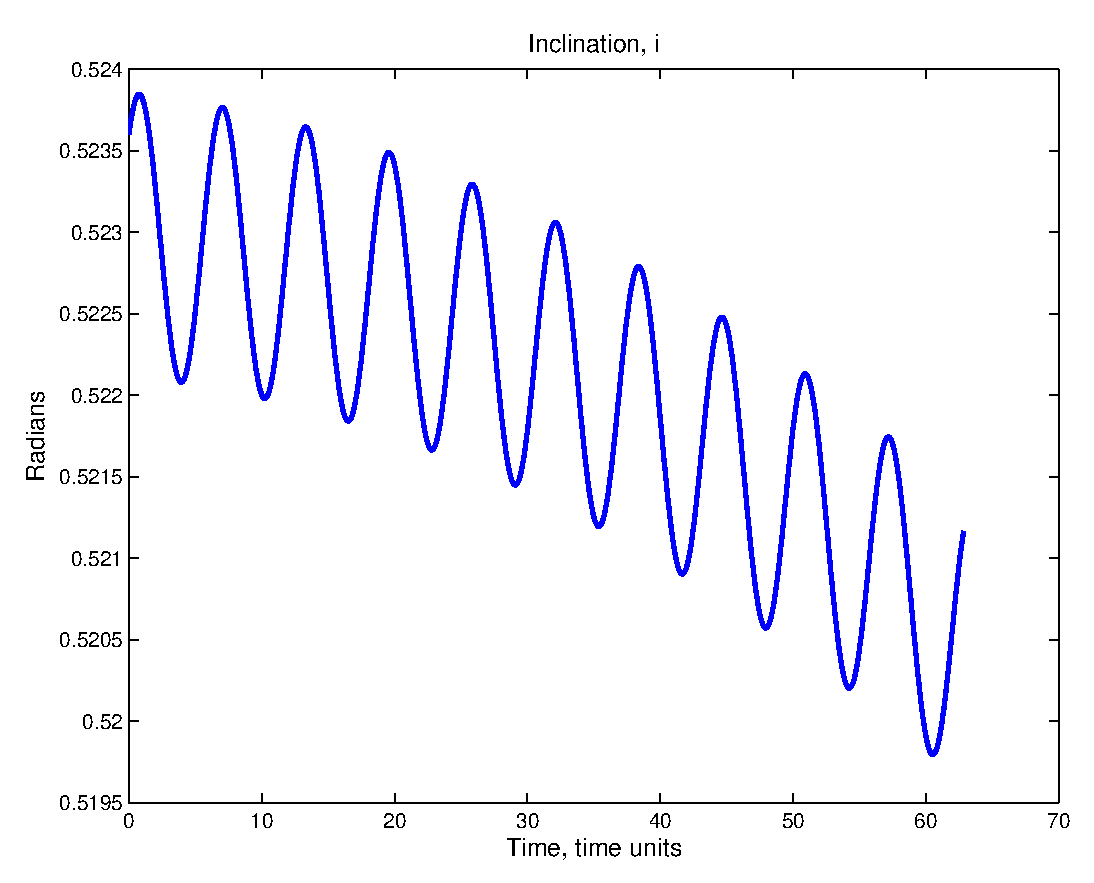
\includegraphics[width = 7.5cm]{Figures/P15_i.eps}
		}
		\subfigure[Argument of periapsis]{
			\includegraphics[width = 7.5cm]{Figures/P15_w.eps}
		}
		\subfigure[RAAN]{
			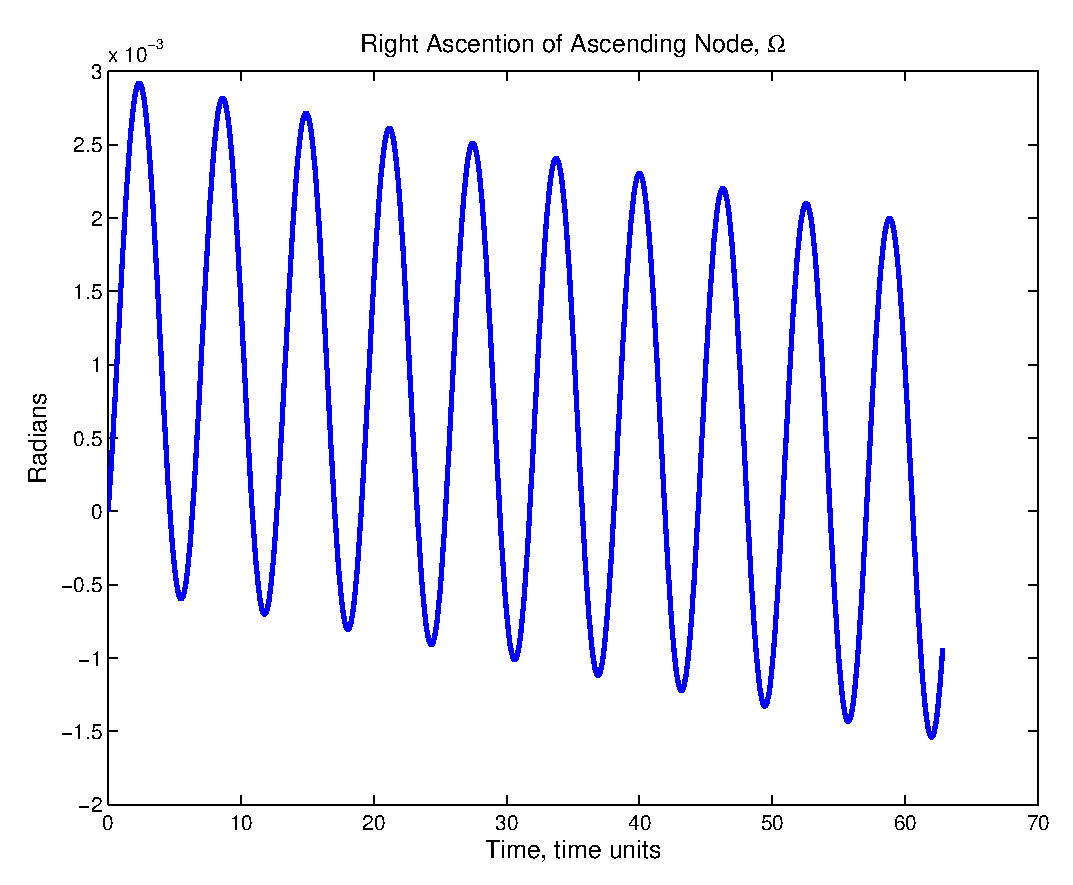
\includegraphics[width = 7.5cm]{Figures/P15_RAAN.eps}
		}
		\subfigure[True anomaly]{
			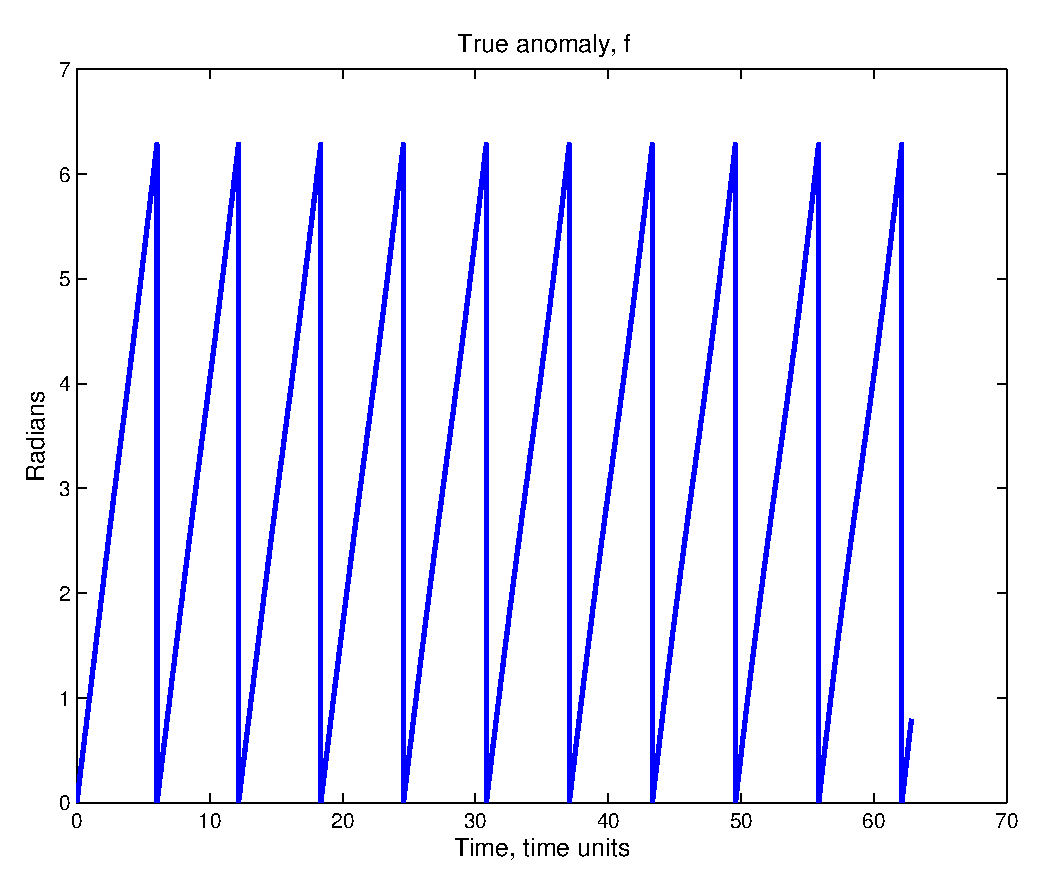
\includegraphics[width = 7.5cm]{Figures/P15_f.eps}
		}
	\caption{Simulation results, orbital elements }
		\label{fig:P15_OE}
	\end{figure}	

	\begin{figure}[H]
		\centering
		\subfigure[Euler angles wrt LVLH]{
			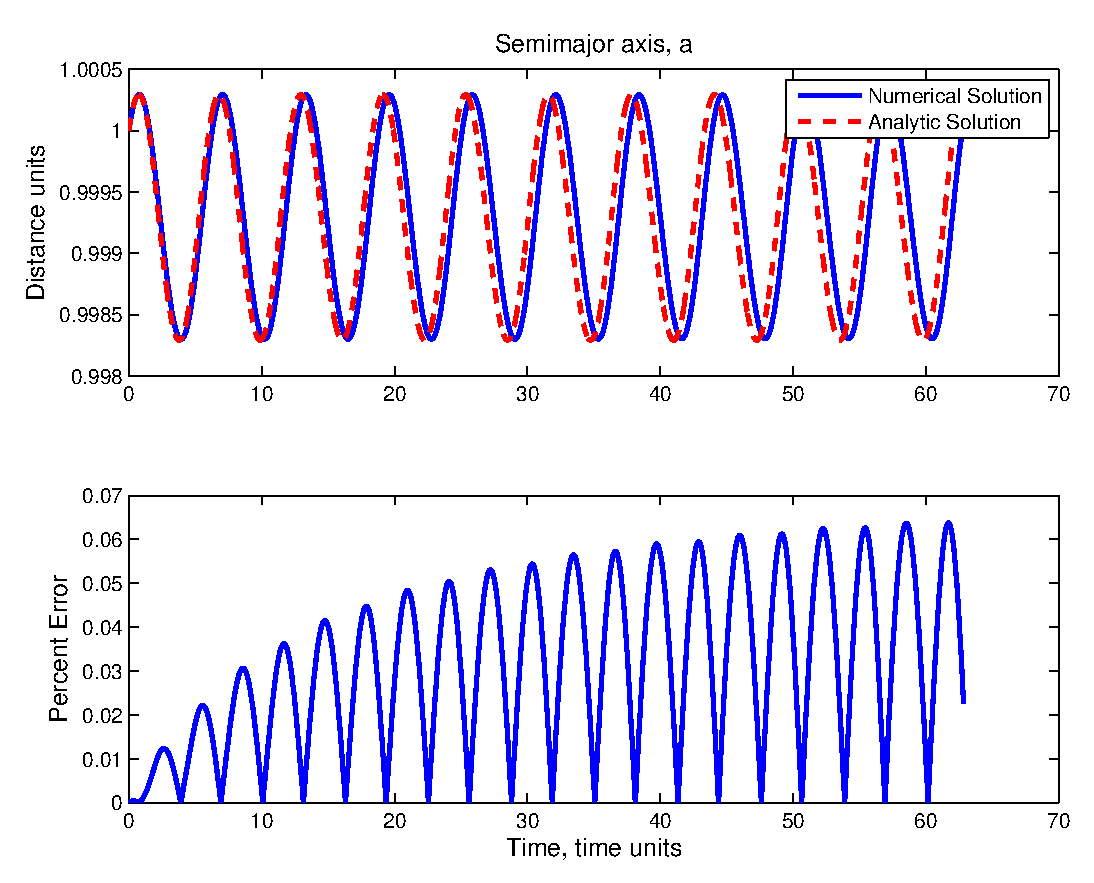
\includegraphics[width = 12cm]{Figures/P15_SMA.eps}
		}
		\subfigure[Body Rates]{
			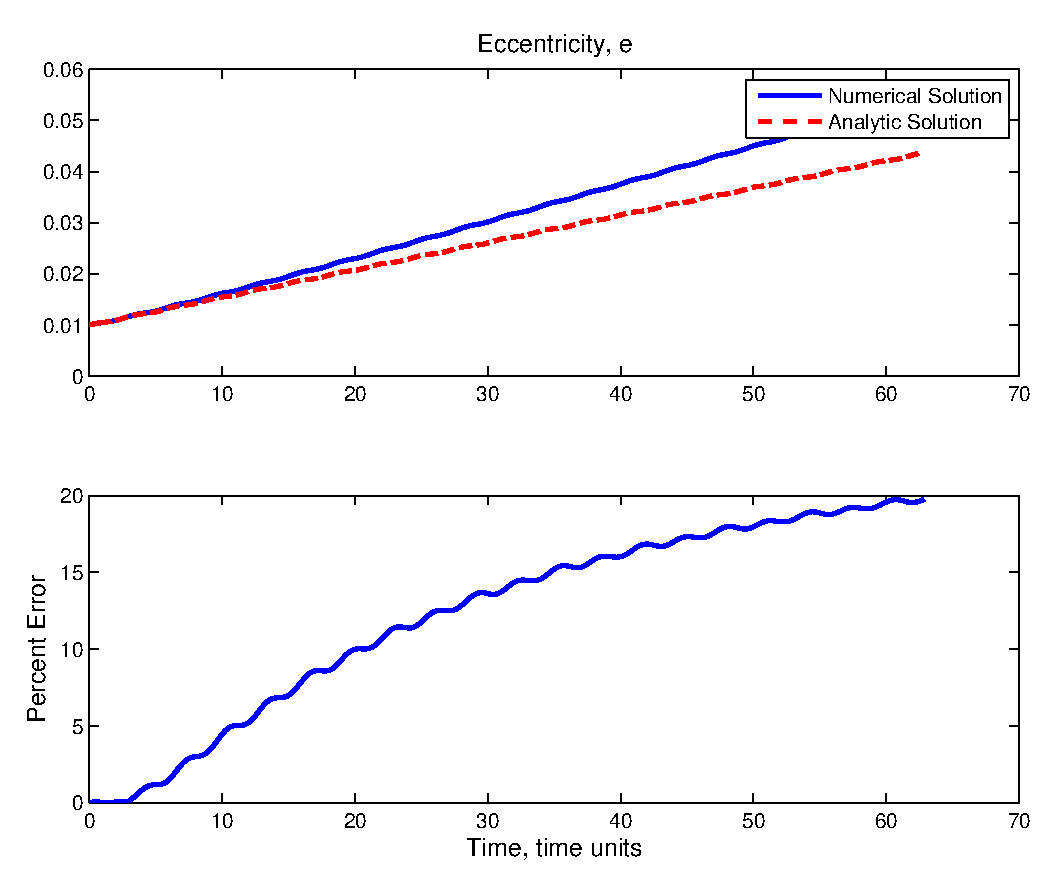
\includegraphics[width = 12cm]{Figures/P15_Ecc.eps}
		}
	\caption{Simulation results,  $a$ and $e$}
		\label{fig:P15_ae}

	\end{figure}

The argument of periapsis shows the most change of the orbit-orientation angles. While inclination and RAAN have secular change as well, they are quite small compared to $\omega$. Although $a$ does not experience secular change, the numerical solution diverges a small amount from the analitical solution. The divergence starts small and grows, likely due to the cos$\omega$ and sin$\omega$ terms changing. The eccentricity experiences the largest error between the two solutions. Since there is secular change in $e$, the change predicted by $\Delta e$ becomes less accurate as time goes on and $e$ grows over each orbit.

\subsection{}
The short period term $\bar{\Delta a}$ is as follows:
	\begin{equation} 
\begin{aligned}
\bar{\Delta a} &= \frac{1}{2\pi}\int_{0}^{2\pi}\Delta a(E) dM =\frac{1}{2\pi}\int_{0}^{2\pi}\frac{2\sqrt{1-e^2}\textup{sin}i\,a_s}{n^2}\left [ \sqrt{1-e^2}\textup{cos}\omega \textup{sin}E -\textup{sin}\omega\left ( 1-\textup{cos}E \right ) \right ]\left ( 1-e\textup{cos}E \right )dE \\
&= \frac{\sqrt{1-e^2}\textup{sin}i\,a_s}{\pi\,n^2}\int_{0}^{2\pi} \left [ \sqrt{1-e^2}\textup{cos}\omega \textup{sin}E -\sqrt{1-e^2}e\textup{cos}\omega \textup{cos}E\textup{sin}E -\textup{sin}\omega +e\textup{sin}\omega \textup{cos}E +\textup{sin}\omega \textup{cos}E-e\textup{sin}\omega \textup{cos}^2E \right ]dE \\
&=-\frac{2\sqrt{1-e^2}\textup{sin}i\textup{sin}\omega\,a_s}{n^2}
 \end{aligned}
	\end{equation} 

The short period term $\bar{\Delta e}$ is as follows:
	\begin{equation} 
\begin{aligned}
\bar{\Delta e} = \frac{1}{2\pi}\int_{0}^{2\pi}\left (\Delta e(E) -\frac{1}{n}\bar{\dot{e}}M \right ) dM 
 \end{aligned}
\label{eqn:overall_debar}
	\end{equation} 

Breaking up the integral into two parts, we can solve for the first:
	\begin{equation} 
\begin{aligned}
\frac{1}{2\pi}\int_{0}^{2\pi}\Delta e(E)dM = \frac{1}{2\pi}\int_{0}^{2\pi}&\frac{\sqrt{1-e^2}\textup{\textup{sin}}i\,a_s}{n^2a} \\ &\left [ \frac{3}{2}\textup{\textup{cos}}\omega E -2e\textup{cos}\omega \textup{sin}E +\frac{1}{4}\textup{cos}\omega \textup{sin}2E-\frac{\sqrt{1-e^2}}{4}\textup{sin}\omega +\frac{\sqrt{1-e^2}}{4}\textup{sin}\omega \textup{cos}2E\right ]\left ( 1-e\textup{cos}E \right )dE
 \end{aligned}
	\end{equation} 

Using the double-angle identities, distributing, and using Eqns \ref{eqn:cosInt}, \ref{eqn:sinInt}, \ref{eqn:cos2Int}, \ref{eqn:cosSinInt}, and \ref{eqn:EInt}:
	\begin{equation} 
 \begin{aligned}
\frac{1}{2\pi}\int_{0}^{2\pi}\Delta e(E)dM = \frac{1}{2\pi}\int_{0}^{2\pi}&\frac{\sqrt{1-e^2}\textup{\textup{sin}}i\,a_s}{n^2a} \\ &\left [ \frac{3}{2}\textup{\textup{cos}}\omega E -2e\textup{cos}\omega \textup{sin}E +\frac{2}{4}\textup{cos}\omega \textup{sin}E\textup{cos}E-\frac{\sqrt{1-e^2}}{4}\textup{sin}\omega +\frac{\sqrt{1-e^2}}{4}\textup{sin}\omega \left (1-2\textup{sin}^2E  \right )\right ]\left ( 1-e\textup{cos}E \right )dE
 \end{aligned}
	\end{equation} 
	\begin{equation} 
\begin{aligned}
\frac{1}{2\pi}\int_{0}^{2\pi}\Delta e(E)dM = \frac{1}{2\pi}\int_{0}^{2\pi}&\frac{\sqrt{1-e^2}\textup{\textup{sin}}i\,a_s}{n^2a} \\ &\left [ \frac{3}{2}\textup{\textup{cos}}\omega E -2e\textup{cos}\omega \textup{sin}E +\frac{1}{2}\textup{cos}\omega \textup{sin}E\textup{cos}E +\frac{\sqrt{1-e^2}}{2}\textup{sin}\omega \textup{sin}^2E  \right ]\left ( 1-e\textup{cos}E \right )dE
 \end{aligned}
	\end{equation} 
	\begin{equation} 
\begin{aligned}
\frac{1}{2\pi}\int_{0}^{2\pi}\Delta e(E)dM &= \frac{1}{2\pi}\frac{\sqrt{1-e^2}\textup{\textup{sin}}i\,a_s}{n^2a} \int_{0}^{2\pi}\left [ \frac{3}{2}\textup{cos}\omega E -\frac{\sqrt{1-e^2}}{2}\textup{sin}\omega \textup{sin}^2E \right ]dE \\
 &= \frac{\sqrt{1-e^2}\textup{\textup{sin}}i\,a_s}{n^2a} \left [\frac{3\pi}{2}\textup{cos}\omega -\frac{\sqrt{1-e^2}}{4}\textup{sin}\omega \right ]
 \end{aligned}
\label{eqn:shortPeriod_e_p1}
	\end{equation} 

Now for the second part:

	\begin{equation} 
\begin{aligned}
\frac{1}{2\pi n}\int_{0}^{2\pi}\dot{e}MdM  &= \frac{1}{2\pi}\frac{\sqrt{1-e^2}\textup{\textup{sin}}i\,a_s}{n^2a} \int_{0}^{2\pi}\left [  \textup{cos}\omega +\textup{cos}(\omega +f )\frac{(e+\textup{cos}f)}{1+e\textup{cos}f} \right ]MdM \\ 
 &=\frac{1}{2\pi}\frac{\sqrt{1-e^2}\textup{\textup{sin}}i\,a_s}{n^2a}\left [ 2\pi^2\textup{cos}\omega + \int_{0}^{2\pi} \left ( \textup{cos}\omega \textup{cos}E -e\textup{cos}\omega \textup{cos}E -\sqrt{1-e^2}\textup{sin}\omega \textup{sin}E \right )\textup{cos}E\left ( E-e\textup{sin}E \right )dE\right ]
\end{aligned}
\label{eqn:shortPeriod_e_p21}
	\end{equation} 

The remaining integral becomes:
	\begin{equation} 
\begin{aligned}
& \int_{0}^{2\pi} \left ( \textup{cos}\omega \textup{cos}E -e\textup{cos}\omega \textup{cos}E -\sqrt{1-e^2}\textup{sin}\omega \textup{sin}E \right )\textup{cos}E\left ( E-e\textup{sin}E \right )dE \\
 &= \int_{0}^{2\pi} \left ( \textup{cos}\omega \textup{cos}^2E -e\textup{cos}\omega \textup{cos}^2E -\sqrt{1-e^2}\textup{sin}\omega \textup{sin}E\textup{cos}E \right )\left ( E-e\textup{sin}E \right )dE \\
 &= \pi^2\textup{cos}\omega + \frac{\pi \sqrt{1-e^2}}{2}\textup{sin}\omega \\ 
\end{aligned}
\label{eqn:shortPeriod_e_p22}
	\end{equation} 

Combining Eqns \ref{eqn:shortPeriod_e_p21} and \ref{eqn:shortPeriod_e_p22}:
	\begin{equation} 
\begin{aligned}
\frac{1}{2\pi n}\int_{0}^{2\pi}\dot{e}MdM &=\frac{1}{2\pi}\frac{\sqrt{1-e^2}\textup{\textup{sin}}i\,a_s}{n^2a}\left [ 3\pi^2\textup{cos}\omega + \frac{\pi \sqrt{1-e^2}}{2}\textup{sin}\omega \right ]
\end{aligned}
\label{eqn:shortPeriod_e_p2}
	\end{equation} 

And combining Eqns \ref{eqn:shortPeriod_e_p1} and \ref{eqn:shortPeriod_e_p2} into \ref{eqn:overall_debar} yield:

	\begin{equation} 
\begin{aligned}
\bar{\Delta e} = \frac{1}{2\pi}\int_{0}^{2\pi}\left (\Delta e(E) -\frac{1}{n}\bar{\dot{e}}M \right ) dM =0
 \end{aligned}
\label{eqn:overall_debar}
	\end{equation} 


The results of the short-period averaging are shown in Figure \ref{fig:SimResults} below.
	\begin{figure}[H]
		\centering
		\subfigure[Semimajor axis short-period averages]{
			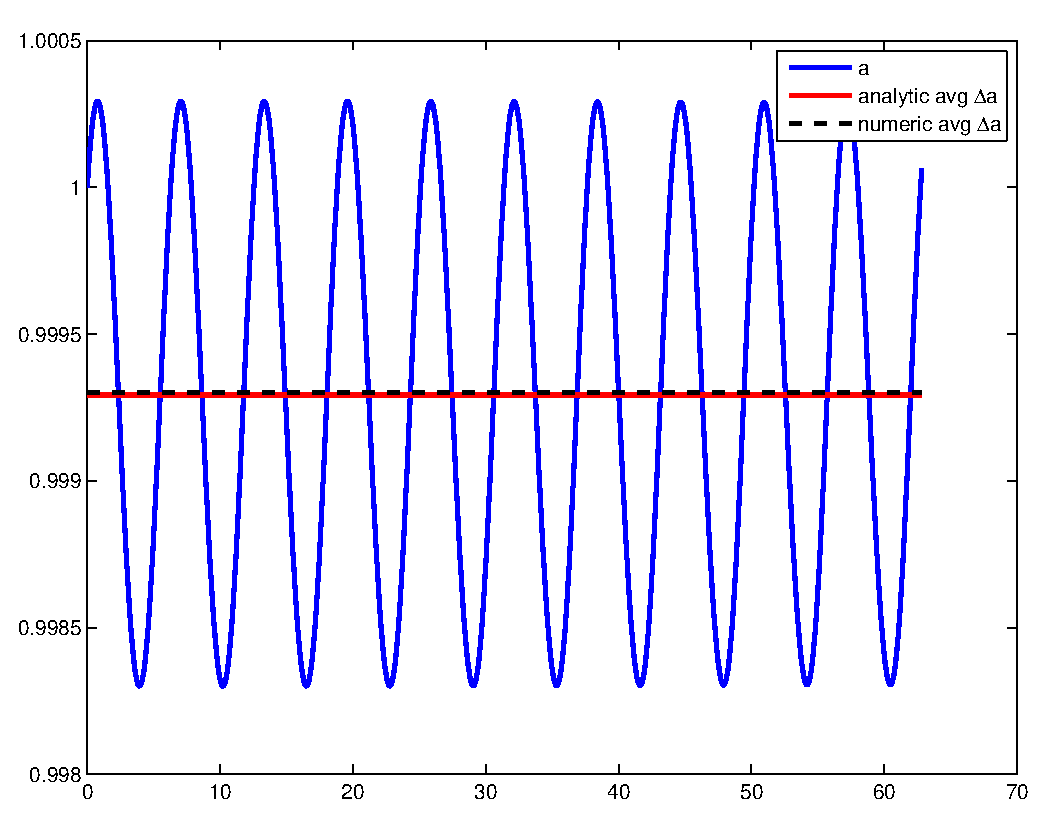
\includegraphics[width = 10cm]{Figures/P15_avg_a.eps}
		}
		\subfigure[Eccentricity short-period averages]{
			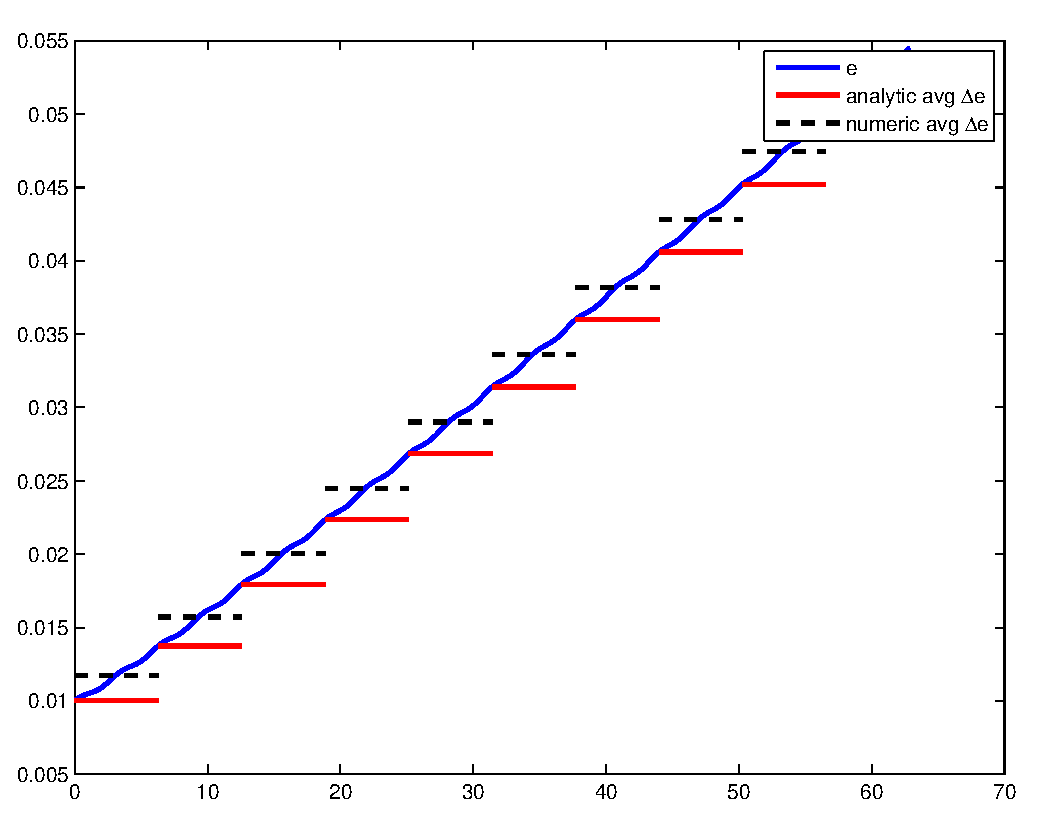
\includegraphics[width = 10cm]{Figures/P15_avg_e.eps}
		}
	\caption{Average short-period changes }
		\label{fig:SimResults}
	\end{figure}

As expected, the $\bar{\Delta a}$ in the numerical and analytical solutions are very close since there is no secular change in $a$. However, the $\bar{\Delta e}$ solutions, taken at the beginning of each orbit, differ quite a bit. This means that $e$ \textit{only} changes secularly.
	



\bibliographystyle{aiaa}   % Number the references.
\bibliography{ASEN6080ProjectBib}   % Use references.bib to resolve the labels.

%    \section{Appendix B}
%This appendix contains all Matlab code used by the authors to analyize their data.
%    
%    \lstset{language=Matlab,%
%    	%basicstyle=\color{red},
%    	breaklines=true,%
%    	morekeywords={matlab2tikz},
%    	keywordstyle=\color{blue},%
%    	morekeywords=[2]{1}, keywordstyle=[2]{\color{black}},
%    	identifierstyle=\color{black},%
%    	stringstyle=\color{mylilas},
%    	commentstyle=\color{mygreen},%
%    	showstringspaces=false,%without this there will be a symbol in the places where there is a space
%    	numbers=left,%
%    	numberstyle={\tiny \color{black}},% size of the numbers
%    	numbersep=9pt, % this defines how far the numbers are from the text
%    	emph=[1]{for,end,break},emphstyle=[1]\color{red}, %some words to emphasise
%    	%emph=[2]{word1,word2}, emphstyle=[2]{style},   
%    }
    
%    \lstinputlisting{ASEN5090_ecef2azelrange.m}
%    \vspace{5mm}
%    
%    \lstinputlisting{ASEN5090_GPSvis.m}
%    \vspace{5mm}
%\lstinputlisting{HW5_rel_err.m}
%\vspace{5mm}
%\lstinputlisting{import_gps_data.m}
%\vspace{5mm}
%\lstinputlisting{datenum8601.m}
%\vspace{5mm}
%\lstinputlisting{lab_err_plots.m}
%\vspace{5mm}
	
\end{document}

% - Release $Name:  $ -
